\documentclass[aps,prd,reprint,onecolumn,superscriptaddress,nofootinbib]{revtex4-2}
\usepackage{amsmath,amssymb,graphicx,booktabs}
\usepackage[T1]{fontenc}
\begin{document}
\title{Structured finite-window response sensitivity in correlated Hubble dipoles}
\author{Anonymous research draft}
\noaffiliation
\date{25 October 2026}
\begin{abstract}
Four retained redshift-window dipoles carry a 12-component correlated discrepancy after fitting a bulk response and constant directional rate. We ask how much of this discrepancy can be moved by three prespecified finite-window response classes. Under the retained Gaussian working covariance, the baseline quadratic discrepancy is $23.3967$, above the fixed six-degree 95\% reference $12.5916$. A depth-slope response leaves an irreducible $15.3160$ and cannot reach that reference at any coefficient budget. An FP-composition proxy reaches it at a joint dimensionless coefficient radius $5.7509$; a six-column combination reaches it at $1.5897$. These are exact finite-dimensional sensitivity budgets for declared designs, not estimates of calibration error. We derive the image ellipsoid, its support and attainment, and the minimum-budget crossing including an irreducible-floor equality case.
\end{abstract}
\maketitle

\section{Retained carrier and physical question}

The saved four-window analysis represents each angular-rate estimator by a monopole, three Cartesian dipole coordinates, and five signed symmetric trace-free coordinates in ICRS J2000. The centers are $z_w=(0.025,0.040,0.060,0.080)$ with saved width $h=0.012$. Its full 36-by-36 joint covariance connects axes and windows, including shared groups. We extract the marginal 12-by-12 dipole covariance $C$ and window-major signed dipoles $y$; no conditioning on measured monopole or STF coordinates is performed. The complete physical coefficient carrier and source covariance are retained in the accompanying \texttt{source\_carrier.json}, alongside the extracted $y,C$ and response matrices \cite{h03,physical}. This extraction does not replace those tensors by a scalar.

The retained estimator is a finite weighted angular-rate fit, $cz_i=d_{{\rm DM},i}[H_w+\mathbf D_w\cdot\mathbf n_i+\mathbf n_i^{\mathsf T}Q_w\mathbf n_i]$. Its coefficients are in ${\rm km\,s^{-1}\,Mpc^{-1}}$; they are not themselves physical expansion coefficients. The source contains 35,970 groups, assumes a diagonal row-scatter working law, and leaves common calibration, peculiar-velocity and selection covariance unmeasured. The experiment here consumes only the saved statistics. It does not refit a catalogue or infer an observer-frame or cosmographic transfer.

Let $R$ stack the saved nine-by-three bulk-velocity dipole response blocks, with units ${\rm Mpc}^{-1}$, and let $G=\mathbf 1_4\otimes I_3$. The six-column baseline $X=[R,G]$ has full rank. Its model is
\begin{equation}
 y=Rb+Gd+D\eta+e,\qquad e\sim N(0,C)\quad\text{(retained working law)}.
 \label{eq:model}
\end{equation}
Here $b$ is in ${\rm km\,s^{-1}}$; $d,y,e$ are in ${\rm km\,s^{-1}\,Mpc^{-1}}$. The coefficient $\eta$ is dimensionless under our chosen $D$. The working Gaussian tail at the baseline is $6.7393\times10^{-4}$, a conditional diagnostic under the saved covariance, not survey-null coverage.

\section{Three fixed response mechanisms}

We specify a rate unit $u_0=1\,{\rm km\,s^{-1}\,Mpc^{-1}}$, a depth coordinate $t_w=(z_w-0.04)/h=(-1.25,0,5/3,10/3)$, and the retained FP distance-weight fractions
\begin{equation}
 p=(0.30371471,0.53491724,0.80241152,0.90188987),\qquad f_w=p_w-p_0.
\end{equation}
For window $w$ and Cartesian component $i$, each response has one coefficient per axis $a$:
\begin{equation}
 (D_z)_{(w,i),a}=u_0t_w\delta_{ia},\quad
 (D_{\rm FP})_{(w,i),a}=u_0f_w\delta_{ia},\quad
 D_{\rm joint}=[D_z,D_{\rm FP}].
 \label{eq:design}
\end{equation}
$D_z$ is a linear finite-center directional-rate slope per saved width. $D_{\rm FP}$ is a dipolar offset modulated by FP composition; subtraction of $p_0$ changes only a constant-rate column already fitted by $G$. The composition fractions do not give a signed distance-modulus calibration derivative. The joint design has six coefficients in depth-first, then FP, Cartesian order. All three are declared before seeing their residual reduction, and none is preferred as a physical error model on that basis. The common coefficient metric for each dimension is $M=I_p$: $\|\eta\|_2\leq\rho$. This is one joint sensitivity budget, not independent axis allowances or an empirical prior.

\section{Projection, ellipsoid and minimum budget}

Write $C=LL^{\mathsf T}$ without jitter, $W=L^{-1}$, $A=WX$, and let $Q_A$ have orthonormal columns spanning $A$. The orthogonal residual projector is $P=I-Q_AQ_A^{\mathsf T}$. With $r=PWy$, $B=PWD M^{-1/2}$, and $\xi=M^{1/2}\eta$, profiling the six signal coefficients reduces Eq.~(\ref{eq:model}) to
\begin{equation}
 T_{\min}(\rho)=\min_{\|\xi\|\leq\rho}\|r-B\xi\|^2,
 \quad T_0=\|r\|^2=23.3967205227. \label{eq:profile}
\end{equation}
The covariance is the complete dipole marginal; using only within-window blocks would produce $T_0=8.92571218$ and change the question. We retain the original six-degree reference $\tau=\chi^2_{6,0.95}=12.5915872437$ after minimizing over $\xi$. Replacing its degree count by $12-\operatorname{rank}[X,D]$ would create a different working-law test.

The image $\mathcal E_\rho=\{B\xi:\|\xi\|\leq\rho\}$ is generally a degenerate ellipsoid in the 12D whitened space. Cauchy--Schwarz gives its exact support in direction $u$:
\begin{equation}
 h_{\mathcal E_\rho}(u)=\rho\|B^{\mathsf T}u\|,
 \quad \xi_*=\rho\frac{B^{\mathsf T}u}{\|B^{\mathsf T}u\|}\quad(B^{\mathsf T}u\ne0).
 \label{eq:support}
\end{equation}
When $B^{\mathsf T}u=0$, support is zero and $\xi=0$ attains it. A proposed correction $q$ is attainable exactly when $q\in\operatorname{col}B$ and $\|B^+q\|\leq\rho$: the pseudoinverse is the minimum-norm preimage, while adding a kernel vector cannot lower its norm. An unrestricted 12D ball omits the column-space condition.

For the resolved thin singular-value decomposition $B=U\operatorname{diag}(\sigma_i)V^{\mathsf T}$, define $\alpha=U^{\mathsf T}r$ and $r_\perp=r-U\alpha$. The signed $r_\perp$ and all singular vectors are exported with the data. Orthogonality gives the irreducible discrepancy $T_\perp=\|r_\perp\|^2$ and saturation radius $\rho_{\rm sat}=\|\operatorname{diag}(\sigma_i^{-1})\alpha\|$. For $0<\rho<\rho_{\rm sat}$, stationarity of the convex Lagrangian $\|r-B\xi\|^2+\lambda(\|\xi\|^2-\rho^2)$ yields
\begin{align}
 \xi_\lambda&=V\operatorname{diag}\!\left(\frac{\sigma_i}{\sigma_i^2+\lambda}\right)\alpha,
 &\rho^2&=\sum_i\frac{\sigma_i^2\alpha_i^2}{(\sigma_i^2+\lambda)^2},\label{eq:kkt}\\
 T_{\min}(\rho)&=T_\perp+\sum_i\frac{\lambda^2\alpha_i^2}{(\sigma_i^2+\lambda)^2}.
 \label{eq:objective}
\end{align}
The multiplier is positive and unique on the active interval. At zero budget $T_{\min}=T_0$; at or above saturation the minimum-norm solution $B^+r$ attains $T_\perp$. If $B=0$, the discrepancy never moves. Hence the least coefficient budget for $T_{\min}\leq\tau$ is zero when $T_0\leq\tau$, unattainable when $T_\perp>\tau$, and $\rho_{\rm sat}$ when $T_\perp=\tau<T_0$. The last case is finite attainment, including equality. In the strict crossing case $T_\perp<\tau<T_0$, a unique positive multiplier solves Eq.~(\ref{eq:objective}) at $\tau$, with $\rho$ obtained from Eq.~(\ref{eq:kkt}).

For numerical classification, proximity to $\tau$ is not an exact equality identity: a computed floor within $10^{-9}$ of $\tau$ receives a boundary hold and no finite budget unless equality is established analytically. Before resolving the singular spectrum of $B$ relative to its largest value, we compare it with the positive unprojected scale $\|WD\|_{\rm op}$ for $M=I$. This prevents projection roundoff for the exact $D=X$ zero-response control from becoming apparent signal rank. The three reported designs have certified nonzero projected directions and retain the original relative-spectrum rule.

A second budget counts the image $q=\|B\xi\|$, in whitened discrepancy units. Its exact least value for the same threshold inside $\operatorname{col}B$ is
\begin{equation}
 q_{\min}=\sqrt{T_0-T_\perp}-\sqrt{\tau-T_\perp},\qquad T_\perp\leq\tau<T_0.\label{eq:qmin}
\end{equation}
This follows by moving radially toward $U\alpha$ within the image subspace. It differs from the image norm $q_{95}=\|B\xi_{95}\|$ of the least \emph{coefficient} witness. The earlier unrestricted result $\eta_{95}=\sqrt{T_0}-\sqrt\tau=1.2885530$ is an image-space comparator; $\rho$ has different units and geometry. The bound $\rho_{95}\geq\eta_{95}/\|B\|_{\rm op}$ and $q_{95}\geq\eta_{95}$ provide checks.

\section{Finite-window results}

\begin{table}[t]\caption{Conditional finite-window designs. All discrepancies use the complete 12D covariance and the unchanged six-degree working threshold. $\rho_{95}$ is a dimensionless joint coefficient budget; $q_{95}$ is its projected whitened image norm. The depth design has no finite threshold crossing.}\label{tab:budgets}\begin{ruledtabular}\begin{tabular}{lrrrrr}\text{Design}&$\operatorname{rank}B$&$T_\perp$&$\rho_{95}$&$q_{95}$&$\rho_{\rm sat}$\\
Depth slope&3&15.3160&---&---&0.7465\\
FP composition&3&6.6606&5.7509&1.7108&14.5772\\
Joint&6&0.0000&1.5897&2.7480&15.4461\\
\end{tabular}\end{ruledtabular}\end{table}

The depth response has three projected directions and leaves $T_\perp=15.3160>\tau$ even at infinite coefficient radius. The three-column FP proxy leaves $T_\perp=6.6606$ and crosses at $\rho_{95}=5.7509$, with $q_{95}=1.7108$. The six-column joint design spans all six baseline residual directions numerically, leaves a floor below $2\times10^{-28}$, and crosses at $\rho_{95}=1.5897$, with $q_{95}=2.7480$. The large $\rho_{\rm sat}$ values in Table~\ref{tab:budgets} show that crossing and complete removal are distinct events. The joint image-space minimum $q_{\min}=1.2885530$ equals the unrestricted radial comparator because the image spans the six-dimensional residual space; its minimum-coefficient witness follows a different route and has the larger $q_{95}$.

\begin{figure}[t]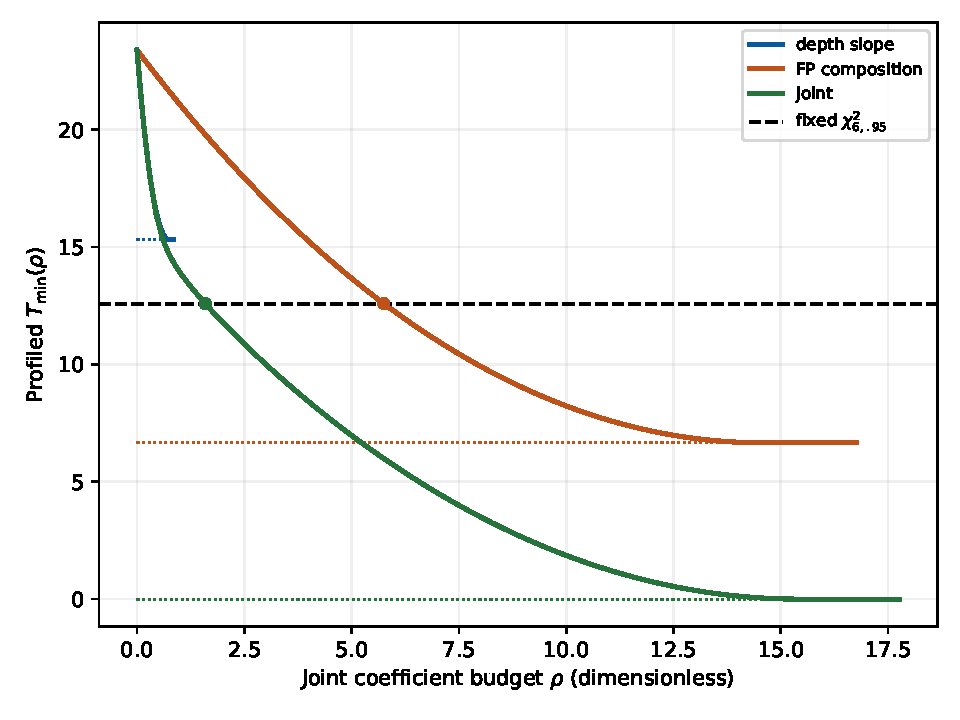
\includegraphics[width=.85\linewidth]{figures/scientific_budget.pdf}\caption{Profiled discrepancy against a \emph{joint} dimensionless coefficient radius for the three fixed finite-window designs. Dots are attained crossings of the unchanged six-degree reference; dotted horizontal lines are the irreducible floors. The depth-slope curve stays above the reference. Generated from the retained 12D covariance in ICRS J2000.}\label{fig:budget}\end{figure}
\begin{figure}[t]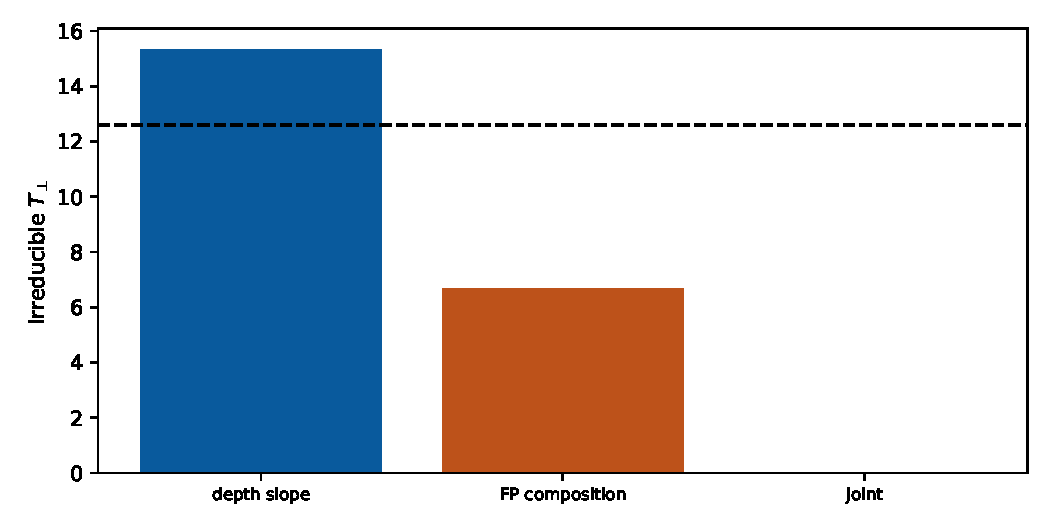
\includegraphics[width=.85\linewidth]{figures/irreducible_floor.pdf}\caption{Exact best attainable discrepancy for each declared projected response subspace. The depth-slope floor exceeds the fixed working threshold. Bars summarize the signed 12-coordinate residual vectors retained in the companion numerical product; they do not encode a physical calibration distribution.}\label{fig:floor}\end{figure}
\begin{figure}[t]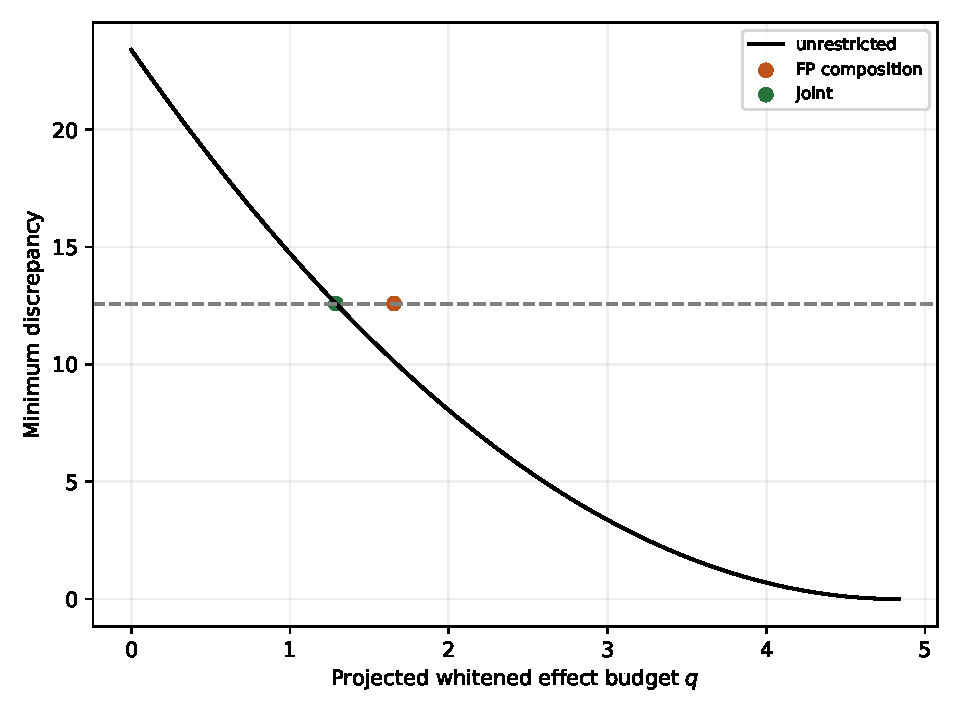
\includegraphics[width=.85\linewidth]{figures/frontier_comparison.pdf}\caption{Unrestricted 12D image-budget frontier $\max(0,\sqrt{T_0}-q)^2$ and the least image radius required by each structure. No depth-slope point exists because its irreducible floor exceeds the threshold. For the FP and joint designs, the plotted minimum-image points are distinct from the coefficient-minimizing image norms $q_{95}$ in Table~\ref{tab:budgets}.}\label{fig:frontier}\end{figure}

The computation exports the full $D$ and $B$ matrices, singular spectra, whitened residual and nonspanning remainder, threshold coefficient vectors, signed corrections, refitted $b,d$, and direct GLS residuals. The direct refits reproduce the fixed threshold within $10^{-8}$. Synthetic checks recover the wrong block-diagonal baseline, zero gain when $D=X$, nonspanning floors at arbitrarily large budgets, finite equality when the floor equals the threshold, the unrestricted radial formula when $D=L$, and invariance under a simultaneous Cartesian rotation. The computation uses the original source hashes and no source reintegration.

\section{Interpretation and required physical input}

These results identify sensitivity of a retained finite-window fit to three explicit response spaces. The FP fractions encode sample composition, not a signed calibration Jacobian; family-deletion dipole norms cannot supply such a derivative. For an actual weighted least-squares estimator $\theta=N^{-1}b$, a physical perturbation $\gamma$ requires $\partial_\gamma\theta=N^{-1}(\partial_\gamma b-(\partial_\gamma N)\theta)$, including any changed distances, design and weights. A source-bound signed window response to named calibration, peculiar-velocity or selection parameters, together with a justified joint bound or law and shared covariance, is needed to interpret $\eta$ as a physical error. The sky, observer and cosmographic transfer, finite remainder and null coverage are likewise open for stronger claims.

The full physical $(x,F,\Pi,Q,G_F)$ object remains undefined here; no filling fraction, exceedance probability, score or depth-gap is zero-filled from this 12D statistic. The result supplies a conditional structured-response frontier for a later model-dependent analysis. It does not alter the original 42-node acceptance status or identify a Bianchi family.

\begin{thebibliography}{2}
\bibitem{h03} Retained H03 source tomography, \texttt{evidence/sources/H03\_SOURCE\_TOMOGRAPHY.json}, SHA-256 \texttt{5d31e2ab4fea682c538c31c15181ae7b07e11efba98b36c66aff6feca88f8326} (2026).
\bibitem{physical} Retained physical-results extraction, \texttt{evidence/output/physical\_results.json}, SHA-256 \texttt{25342649e30a8d631a5364002ae39ebffae0a5d92e1e4ad25c9e2f8dfe9362cc} (2026).
\end{thebibliography}
\end{document}
